\documentclass[12pt,letterpaper]{article}
\usepackage{graphicx,textcomp}
\usepackage{natbib}
\usepackage{setspace}
\usepackage{fullpage}
\usepackage{color}
\usepackage[reqno]{amsmath}
\usepackage{amsthm}
\usepackage{fancyvrb}
\usepackage{amssymb,enumerate}
\usepackage[all]{xy}
\usepackage{endnotes}
\usepackage{lscape}
\newtheorem{com}{Comment}
\usepackage{float}
\usepackage{hyperref}
\newtheorem{lem} {Lemma}
\newtheorem{prop}{Proposition}
\newtheorem{thm}{Theorem}
\newtheorem{defn}{Definition}
\newtheorem{cor}{Corollary}
\newtheorem{obs}{Observation}
\usepackage[compact]{titlesec}
\usepackage{dcolumn}
\usepackage{tikz}
\usetikzlibrary{arrows}
\usepackage{multirow}
\usepackage{xcolor}
\newcolumntype{.}{D{.}{.}{-1}}
\newcolumntype{d}[1]{D{.}{.}{#1}}
\definecolor{light-gray}{gray}{0.65}
\usepackage{url}
\usepackage{listings}
\usepackage{color}

\definecolor{codegreen}{rgb}{0,0.6,0}
\definecolor{codegray}{rgb}{0.5,0.5,0.5}
\definecolor{codepurple}{rgb}{0.58,0,0.82}
\definecolor{backcolour}{rgb}{0.95,0.95,0.92}

\lstdefinestyle{mystyle}{
	backgroundcolor=\color{backcolour},   
	commentstyle=\color{codegreen},
	keywordstyle=\color{magenta},
	numberstyle=\tiny\color{codegray},
	stringstyle=\color{codepurple},
	basicstyle=\footnotesize,
	breakatwhitespace=false,         
	breaklines=true,                 
	captionpos=b,                    
	keepspaces=true,                 
	numbers=left,                    
	numbersep=5pt,                  
	showspaces=false,                
	showstringspaces=false,
	showtabs=false,                  
	tabsize=2
}
\lstset{style=mystyle}
\newcommand{\Sref}[1]{Section~\ref{#1}}
\newtheorem{hyp}{Hypothesis}

\title{Problem Set 3}
\date{Due: November 12, 2026}
\author{Owen Stidman}


\begin{document}
	\maketitle
	\section*{Instructions}
	\begin{itemize}
		\item Please show your work! You may lose points by simply writing in the answer. If the problem requires you to execute commands in \texttt{R}, please include the code you used to get your answers. Please also include the \texttt{.R} file that contains your code. If you are not sure if work needs to be shown for a particular problem, please ask.
	\item Your homework should be submitted electronically on GitHub.
	\item This problem set is due before 23:59 on Thursday November 12, 2026. No late assignments will be accepted.

	\end{itemize}

		\vspace{.25cm}
	
\noindent In this problem set, you will run several regressions and create an add variable plot (see the lecture slides) in \texttt{R} using the \texttt{incumbents\_subset.csv} dataset. Include all of your code.

	\vspace{.5cm}
\section*{Question 1}
\vspace{.25cm}
\noindent We are interested in knowing how the difference in campaign spending between incumbent and challenger affects the incumbent's vote share. 
	\begin{enumerate}
		\item Run a regression where the outcome variable is \texttt{voteshare} and the explanatory variable is \texttt{difflog}.	\vspace{0.5cm}
		
		I regress \textit{voteshare} on \textit{difflog} using the following commands in R:
		\lstinputlisting[language=R, firstline=55, lastline=57]{PS03_answers_OS.R} 
		
		The "summary" command produces the following output:
		\begin{verbatim}
			Residuals:
			Min       1Q   Median       3Q      Max 
			-0.26832 -0.05345 -0.00377  0.04780  0.32749 
			
			Coefficients:
			Estimate Std. Error t value
			(Intercept)     0.579031   0.002251  257.19
			inc.sub$difflog 0.041666   0.000968   43.04
			Pr(>|t|)    
			(Intercept)       <2e-16 ***
			inc.sub$difflog   <2e-16 ***
			---
			Signif. codes:  
			0 ‘***’ 0.001 ‘**’ 0.01 ‘*’ 0.05 ‘.’ 0.1 ‘ ’ 1
			
			Residual standard error: 0.07867 on 3191 degrees of freedom
			Multiple R-squared:  0.3673,	Adjusted R-squared:  0.3671 
			F-statistic:  1853 on 1 and 3191 DF,  p-value: < 2.2e-16  
		\end{verbatim}
		
		\item Make a scatterplot of the two variables and add the regression line. 	\vspace{0.5cm}
		
		First, I create the scatterplot using the following code:
		\lstinputlisting[language=R, firstline=66, lastline=71]{PS03_answers_OS.R}
		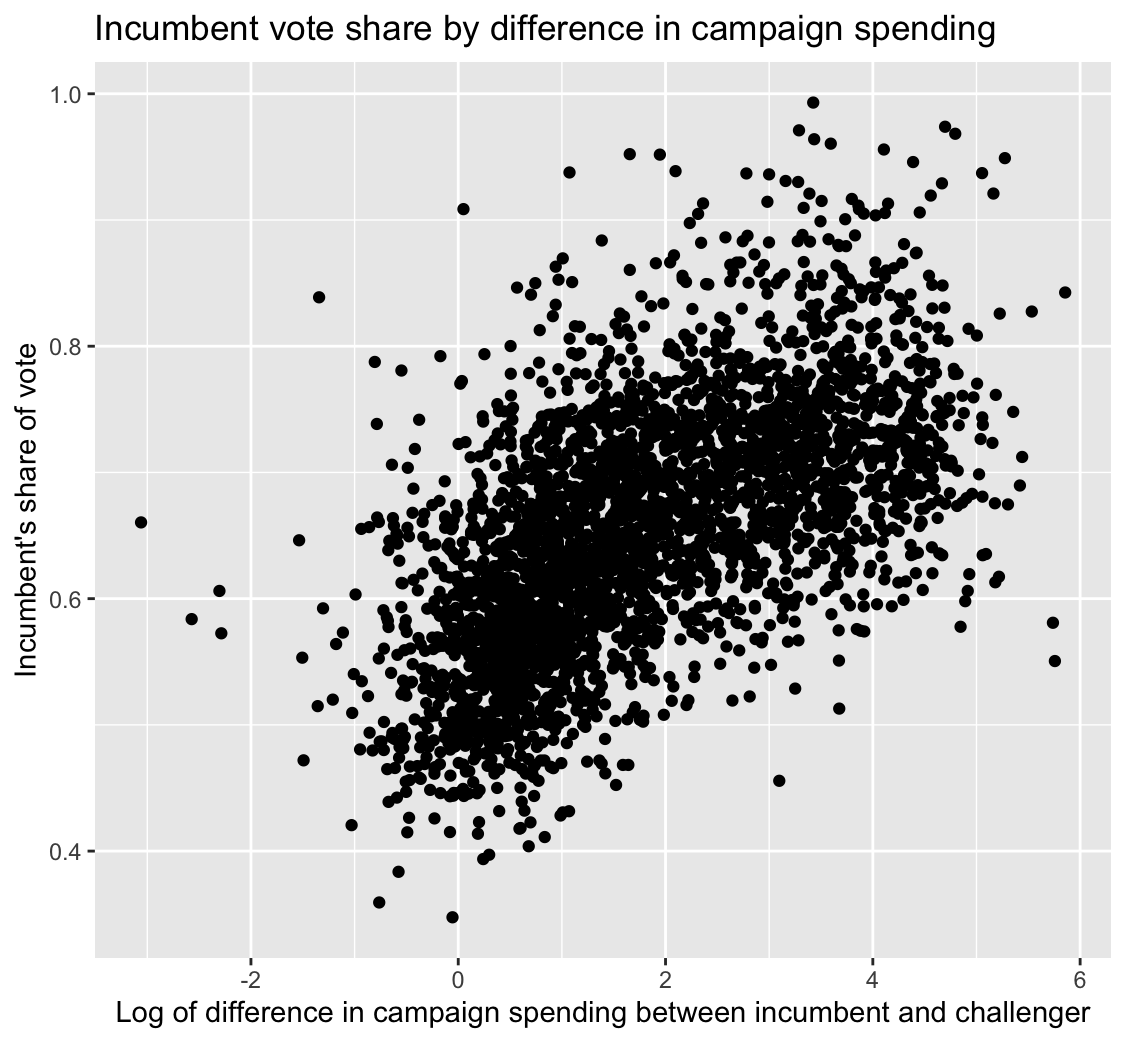
\includegraphics[scale=0.35]{problem1part2graph1}
		
		I add the regression line using this code: 
			\lstinputlisting[language=R, firstline=74, lastline=83]{PS03_answers_OS.R}
		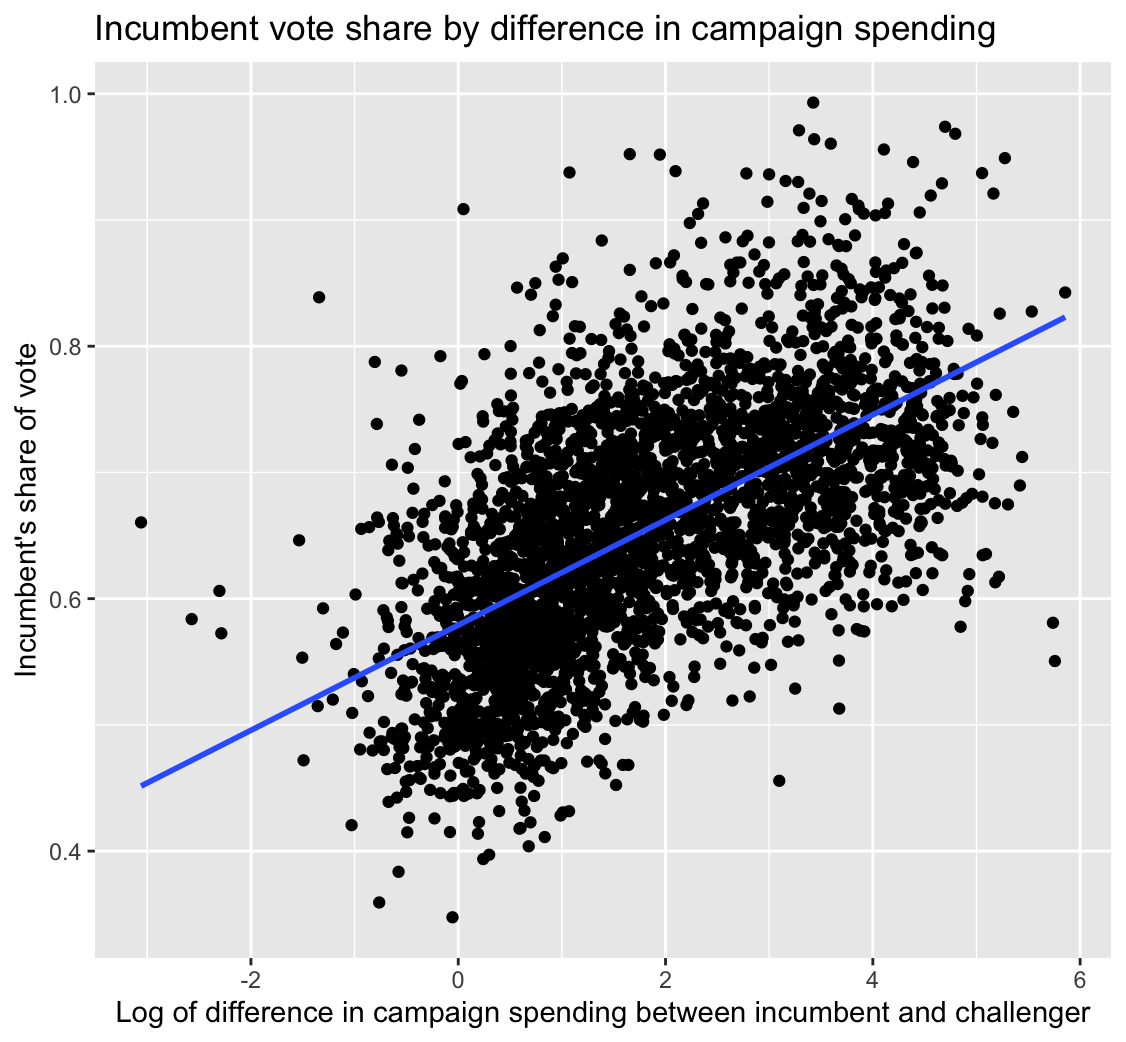
\includegraphics[scale=0.35]{problem1part2graph2}
		
		\item Save the residuals of the model in a separate object.	\vspace{0.5cm}
		
	I save the residuals of the model in a separate object using this command:
		\lstinputlisting[language=R, firstline=91, lastline=91]{PS03_answers_OS.R}
		
		\item Write the prediction equation.
		
		I again run the "summary" command to get the regression coefficient values: 
		
		\lstinputlisting[language=R, firstline=99, lastline=99]{PS03_answers_OS.R}
		
		\begin{verbatim}
			Residuals:
			Min       1Q   Median       3Q      Max 
			-0.26832 -0.05345 -0.00377  0.04780  0.32749 
			
			Coefficients:
			Estimate Std. Error t value
			(Intercept)     0.579031   0.002251  257.19
			inc.sub$difflog 0.041666   0.000968   43.04
			Pr(>|t|)    
			(Intercept)       <2e-16 ***
			inc.sub$difflog   <2e-16 ***
			---
			Signif. codes:  
			0 ‘***’ 0.001 ‘**’ 0.01 ‘*’ 0.05 ‘.’ 0.1 ‘ ’ 1
			
			Residual standard error: 0.07867 on 3191 degrees of freedom
			Multiple R-squared:  0.3673,	Adjusted R-squared:  0.3671 
			F-statistic:  1853 on 1 and 3191 DF,  p-value: < 2.2e-16  
		\end{verbatim}
		
		From the output above:
		
		$\hat{\beta}_0$ (intercept) = 0.579031
		
		$\hat{\beta}_1$ (slope) = 0.041666 
		
		\vspace{.5cm} Therefore:
		
\textbf{		$\hat{voteshare}$ = 0.579031 + 0.041666(\textit{difflog}) + $\epsilon$}
		
	\end{enumerate}
	
\newpage

\section*{Question 2}
\noindent We are interested in knowing how the difference between incumbent and challenger's spending and the vote share of the presidential candidate of the incumbent's party are related.	\vspace{.25cm}
	\begin{enumerate}
		\item Run a regression where the outcome variable is \texttt{presvote} and the explanatory variable is \texttt{difflog}.	\vspace{0.5cm}
		
		I regress \textit{presvote} on \textit{difflog} using the below code:
		\lstinputlisting[language=R, firstline=113, lastline=115]{PS03_answers_OS.R}
		
		The "summary" command produces the following output:
		\begin{verbatim}
			Residuals:
			Min       1Q   Median       3Q      Max 
			-0.32196 -0.07407 -0.00102  0.07151  0.42743 
			
			Coefficients:
			Estimate Std. Error t value Pr(>|t|)    
			(Intercept)     0.507583   0.003161  160.60   <2e-16 ***
			inc.sub$difflog 0.023837   0.001359   17.54   <2e-16 ***
			---
			Signif. codes:  0 ‘***’ 0.001 ‘**’ 0.01 ‘*’ 0.05 ‘.’ 0.1 ‘ ’ 1
			
			Residual standard error: 0.1104 on 3191 degrees of freedom
			Multiple R-squared:  0.08795,	Adjusted R-squared:  0.08767 
			F-statistic: 307.7 on 1 and 3191 DF,  p-value: < 2.2e-16 
		\end{verbatim}
		
		\item Make a scatterplot of the two variables and add the regression line. 	\vspace{.5cm}
		
		First, I create the scatterplot using the following code:
		\lstinputlisting[language=R, firstline=124, lastline=131]{PS03_answers_OS.R}
		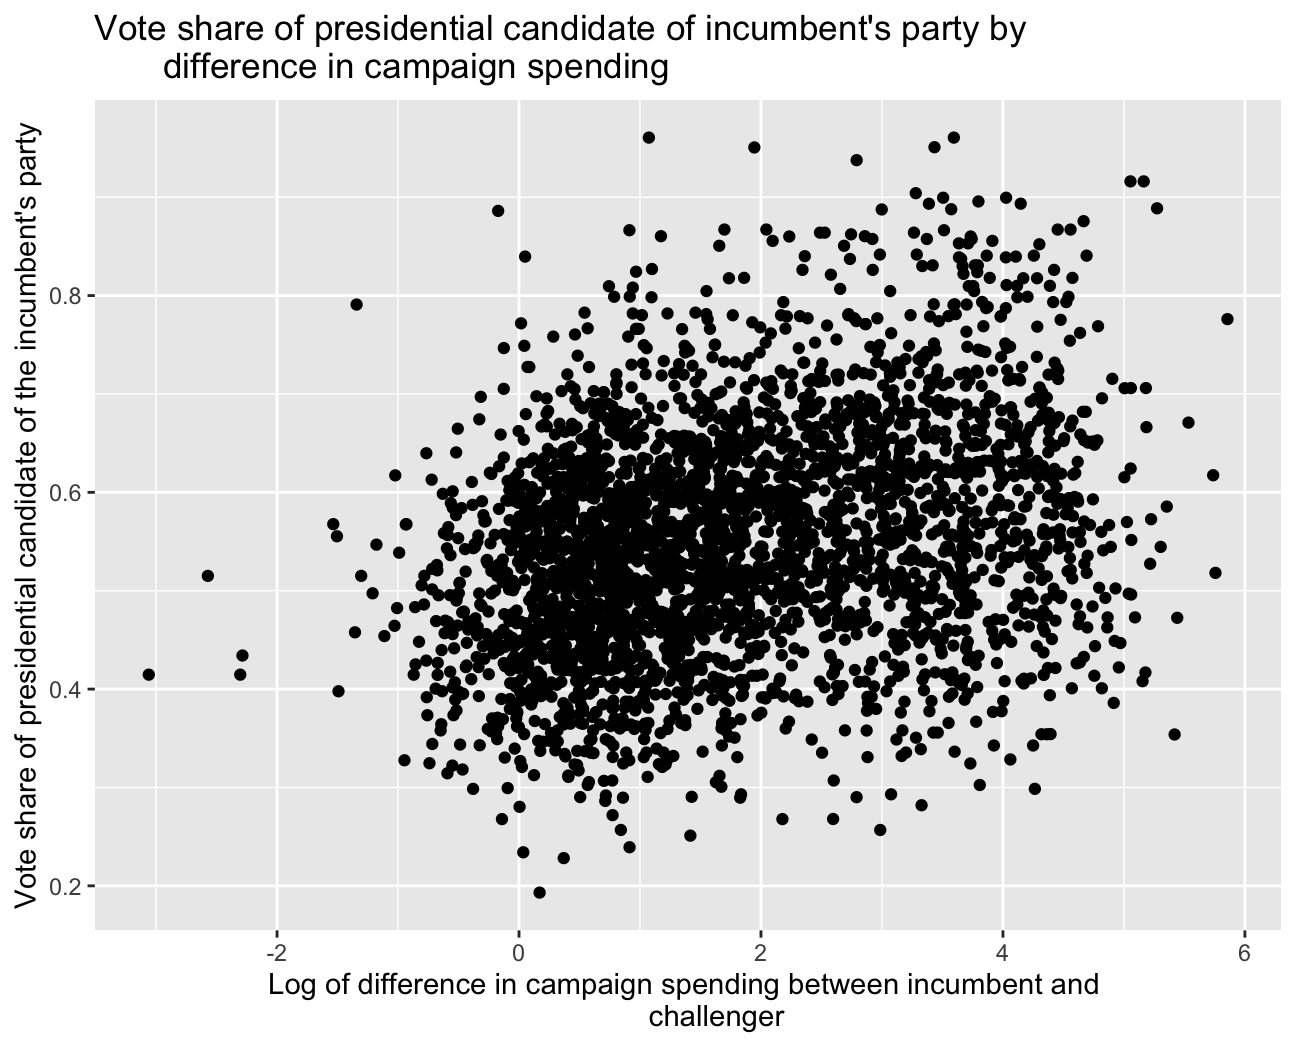
\includegraphics[scale=0.35]{problem2part2graph1}
		
			I add the regression line using this code: 
		\lstinputlisting[language=R, firstline=134, lastline=145]{PS03_answers_OS.R}
		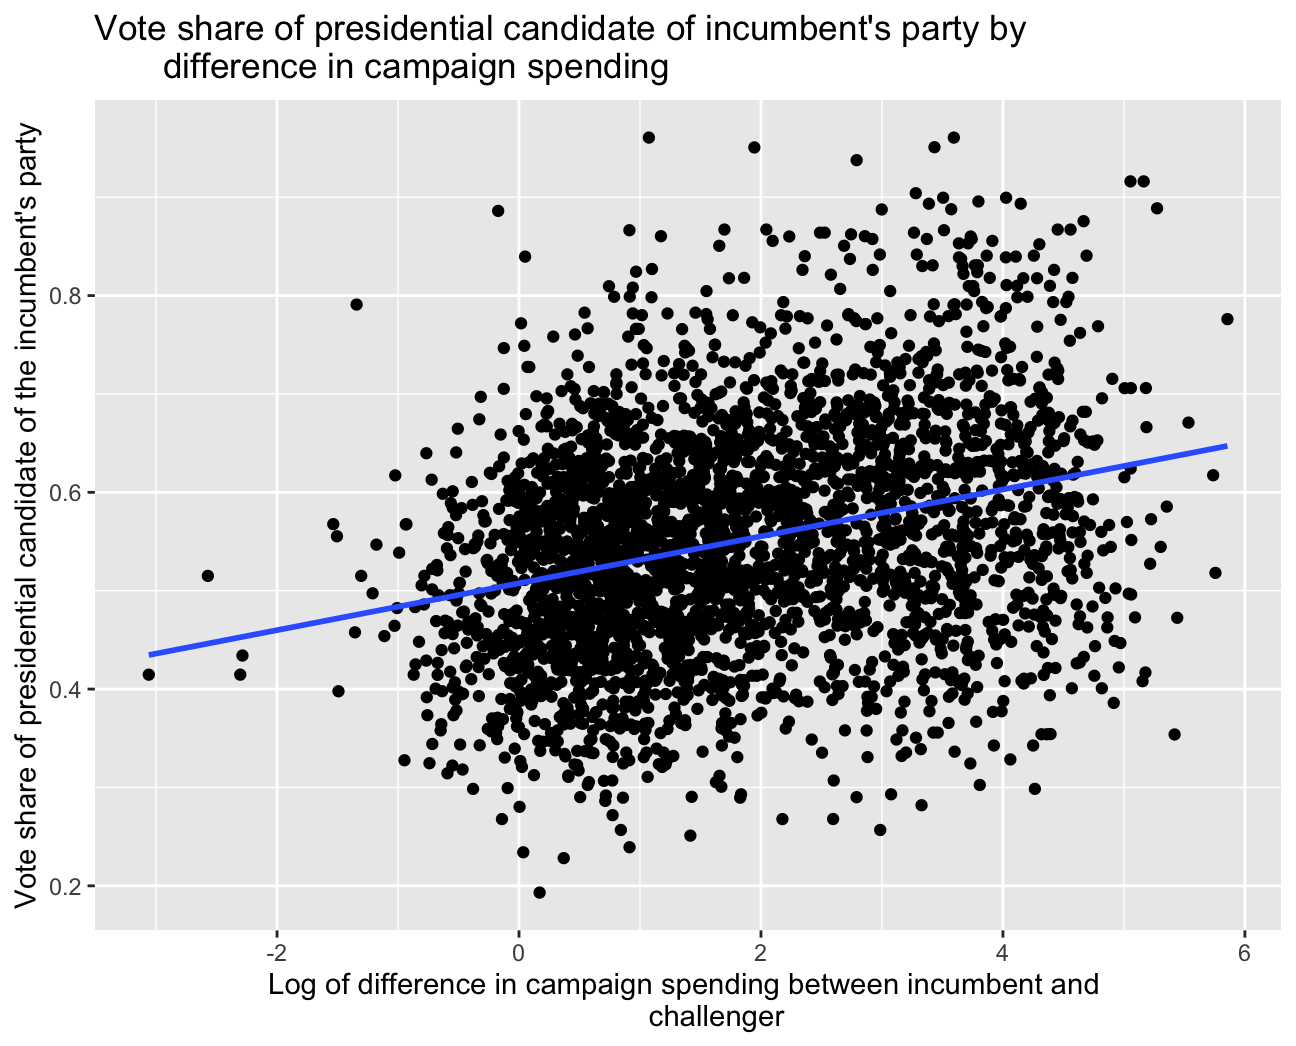
\includegraphics[scale=0.35]{problem2part2graph2}
		
		\item Save the residuals of the model in a separate object.	\vspace{.5cm}
		
			I save the residuals of the model in a separate object using this command:
		\lstinputlisting[language=R, firstline=153, lastline=153]{PS03_answers_OS.R}
		
		\item Write the prediction equation.
		
		I again run the "summary" command to get the regression coefficient values:
		\lstinputlisting[language=R, firstline=161, lastline=161]{PS03_answers_OS.R}
		
		The "summary" command produces the following output:
		\begin{verbatim}
			Residuals:
			Min       1Q   Median       3Q      Max 
			-0.32196 -0.07407 -0.00102  0.07151  0.42743 
			
			Coefficients:
			Estimate Std. Error t value Pr(>|t|)    
			(Intercept)     0.507583   0.003161  160.60   <2e-16 ***
			inc.sub$difflog 0.023837   0.001359   17.54   <2e-16 ***
			---
			Signif. codes:  0 ‘***’ 0.001 ‘**’ 0.01 ‘*’ 0.05 ‘.’ 0.1 ‘ ’ 1
			
			Residual standard error: 0.1104 on 3191 degrees of freedom
			Multiple R-squared:  0.08795,	Adjusted R-squared:  0.08767 
			F-statistic: 307.7 on 1 and 3191 DF,  p-value: < 2.2e-16
		\end{verbatim}
		
			From the output above:
		
		$\hat{\beta}_0$ (intercept) = 0.507583
		
		$\hat{\beta}_1$ (slope) = 0.023837
		
		\vspace{.5cm} Therefore:
		
		\textbf{		$\hat{presvote}$ = 0.579031 + 0.041666(\textit{difflog}) + $\epsilon$}
		
	\end{enumerate}
	
	\newpage	
\section*{Question 3}

\noindent We are interested in knowing how the vote share of the presidential candidate of the incumbent's party is associated with the incumbent's electoral success.
	\vspace{.25cm}
	\begin{enumerate}
		\item Run a regression where the outcome variable is \texttt{voteshare} and the explanatory variable is \texttt{presvote}.
			\vspace{.5cm}
			
			I regress \textit{voteshare} on \textit{presvote} using the following code:
			\lstinputlisting[language=R, firstline=174, lastline=176]{PS03_answers_OS.R}
			
			The "summary" command produces the following output:
			
				\begin{verbatim}
			Residuals:
			Min       1Q   Median       3Q      Max 
			-0.27330 -0.05888  0.00394  0.06148  0.41365 
			
			Coefficients:
			Estimate Std. Error t value Pr(>|t|)    
			(Intercept)      0.441330   0.007599   58.08   <2e-16 ***
			inc.sub$presvote 0.388018   0.013493   28.76   <2e-16 ***
			---
			Signif. codes:  0 ‘***’ 0.001 ‘**’ 0.01 ‘*’ 0.05 ‘.’ 0.1 ‘ ’ 1
			
			Residual standard error: 0.08815 on 3191 degrees of freedom
			Multiple R-squared:  0.2058,	Adjusted R-squared:  0.2056 
			F-statistic:   827 on 1 and 3191 DF,  p-value: < 2.2e-16
			\end{verbatim}
			
		\item Make a scatterplot of the two variables and add the regression line. 
			\vspace{.5cm}
			
			First, I generate the scatterplot using the following code:
			
			\lstinputlisting[language=R, firstline=185, lastline=191]{PS03_answers_OS.R}
			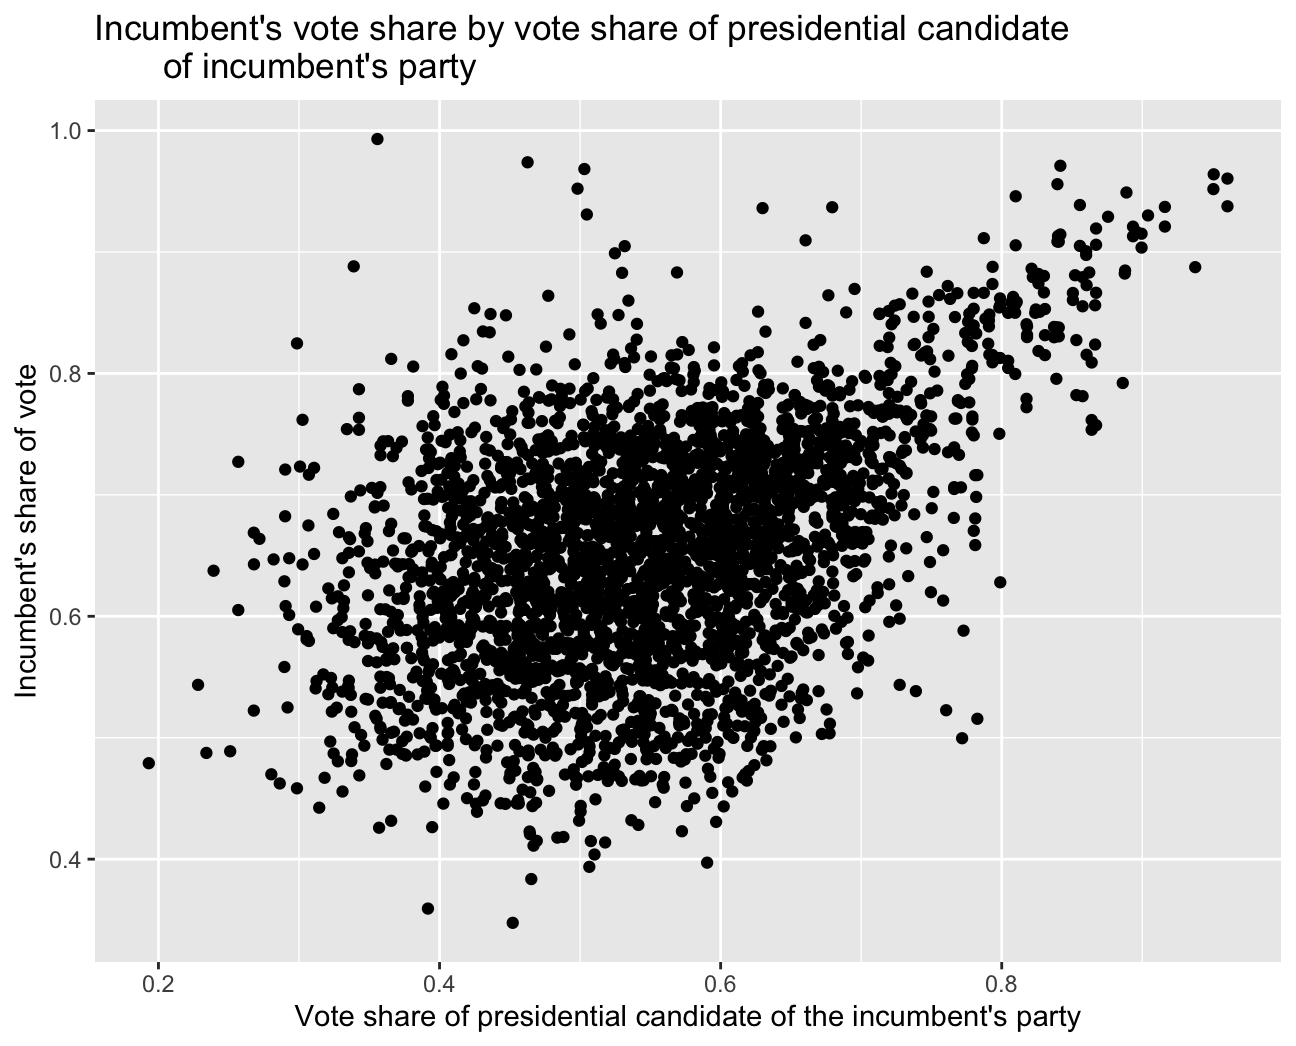
\includegraphics[scale=0.35]{problem3part2graph1}
			
			I add the regression line using the following code:
			
			\lstinputlisting[language=R, firstline=194, lastline=204]{PS03_answers_OS.R}
			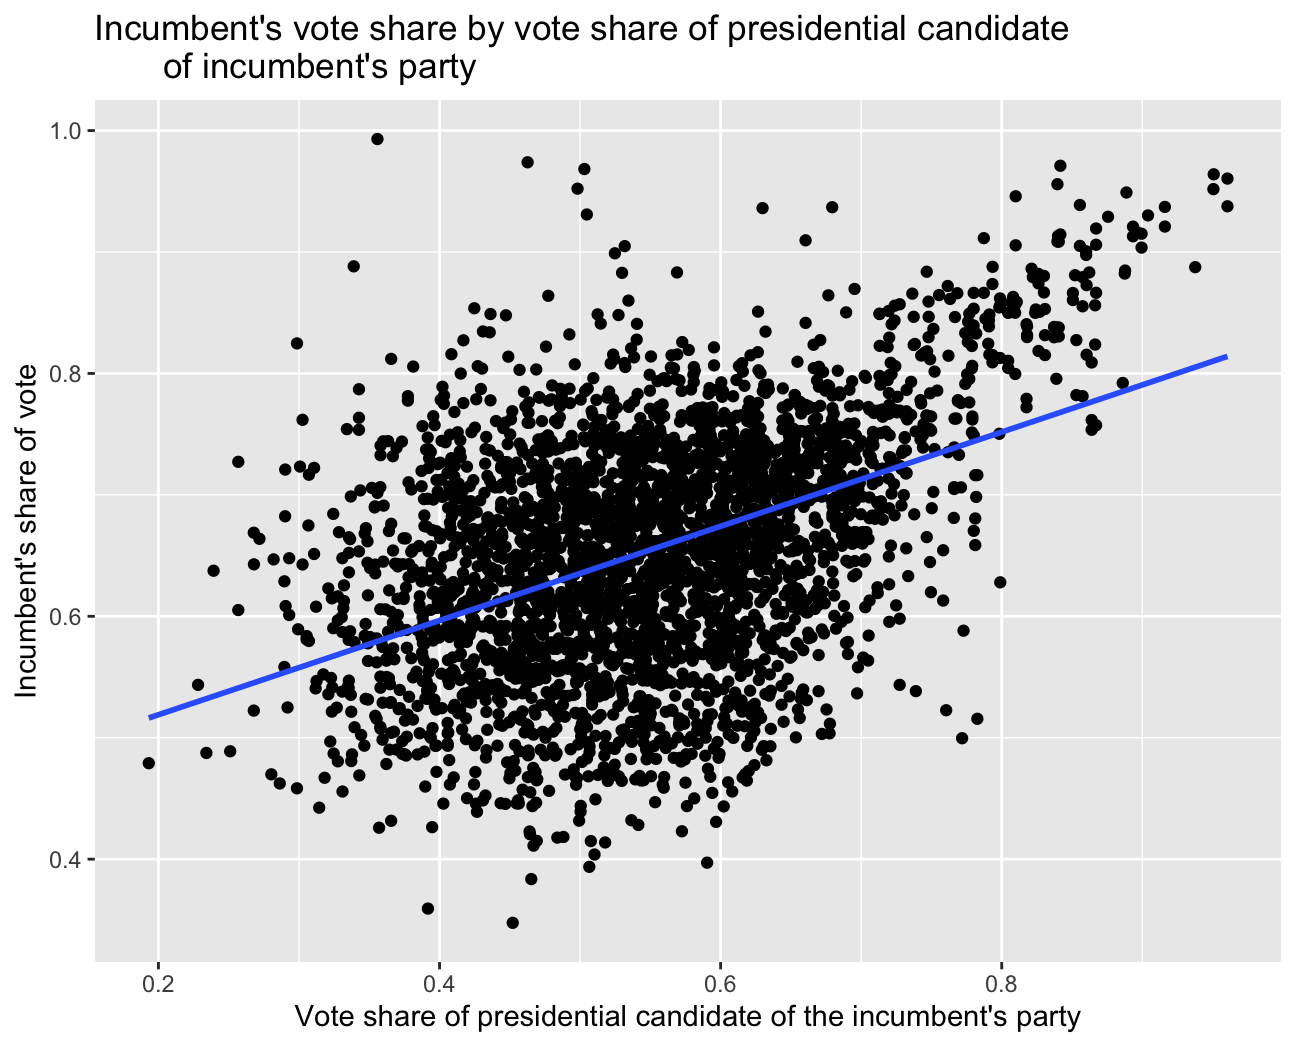
\includegraphics[scale=0.35]{problem3part2graph2}
			
		\item Write the prediction equation.
		
		I again run the "summary" command to get the regression coefficient values:
		
		\lstinputlisting[language=R, firstline=212, lastline=212]{PS03_answers_OS.R}
		
		The "summary" command produces the following output:
		\begin{verbatim}
			Residuals:
			Min       1Q   Median       3Q      Max 
			-0.27330 -0.05888  0.00394  0.06148  0.41365 
			
			Coefficients:
			Estimate Std. Error t value Pr(>|t|)    
			(Intercept)      0.441330   0.007599   58.08   <2e-16 ***
			inc.sub$presvote 0.388018   0.013493   28.76   <2e-16 ***
			---
			Signif. codes:  0 ‘***’ 0.001 ‘**’ 0.01 ‘*’ 0.05 ‘.’ 0.1 ‘ ’ 1
			
			Residual standard error: 0.08815 on 3191 degrees of freedom
			Multiple R-squared:  0.2058,	Adjusted R-squared:  0.2056 
			F-statistic:   827 on 1 and 3191 DF,  p-value: < 2.2e-16
		\end{verbatim}
		
		From the output above:
		
		$\hat{\beta}_0$ (intercept) = 0.441330
		
		$\hat{\beta}_1$ (slope) = 0.388018
		
		\vspace{.5cm} Therefore:
		
		\textbf{		$\hat{voteshare}$ = 0.441330 + 0.388018(\textit{presvote}) + $\epsilon$}
		
	\end{enumerate}
	

\newpage	
\section*{Question 4}
\noindent The residuals from part (a) tell us how much of the variation in \texttt{voteshare} is $not$ explained by the difference in spending between incumbent and challenger. The residuals in part (b) tell us how much of the variation in \texttt{presvote} is $not$ explained by the difference in spending between incumbent and challenger in the district.
	\begin{enumerate}
		\item Run a regression where the outcome variable is the residuals from Question 1 and the explanatory variable is the residuals from Question 2.	\vspace{.5cm}
		
		I regress (the residuals from regressing \textit{voteshare} on \textit{difflog}) on (the residuals from regressing \textit{presvote} on \textit{difflog}) using the following code:
		
				\lstinputlisting[language=R, firstline=228, lastline=230]{PS03_answers_OS.R}
				
		The "summary" command produces the following output:
		
			\begin{verbatim}
		Residuals:
		Min       1Q   Median       3Q      Max 
		-0.25928 -0.04737 -0.00121  0.04618  0.33126 
		
		Coefficients:
		Estimate Std. Error t value Pr(>|t|)    
		(Intercept)                -1.942e-18  1.299e-03    0.00        1    
		residuals_presvote_difflog  2.569e-01  1.176e-02   21.84   <2e-16 ***
		---
		Signif. codes:  0 ‘***’ 0.001 ‘**’ 0.01 ‘*’ 0.05 ‘.’ 0.1 ‘ ’ 1
		
		Residual standard error: 0.07338 on 3191 degrees of freedom
		Multiple R-squared:   0.13,	Adjusted R-squared:  0.1298 
		F-statistic:   477 on 1 and 3191 DF,  p-value: < 2.2e-16
		\end{verbatim}
		
		\item Make a scatterplot of the two residuals and add the regression line. 	\vspace{0.5cm}
		
		First, I generate a scatterplot using the following code:
		
			\lstinputlisting[language=R, firstline=239, lastline=248]{PS03_answers_OS.R}
			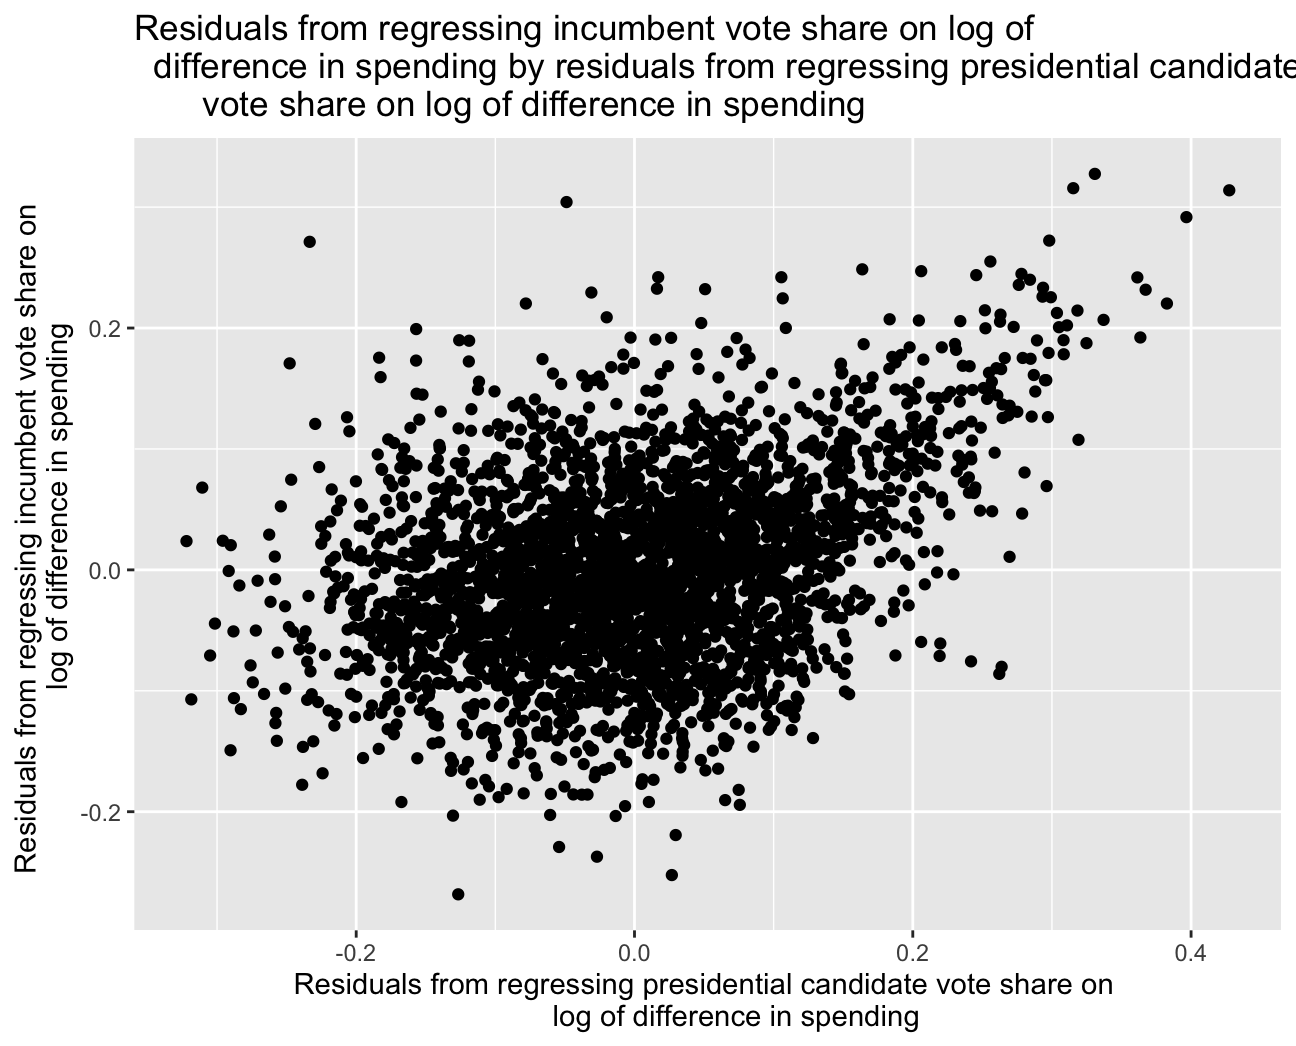
\includegraphics[scale=0.35]{problem4part2graph1}
			
		I add the regression line using the following code:
		
		\lstinputlisting[language=R, firstline=251, lastline=264]{PS03_answers_OS.R}
		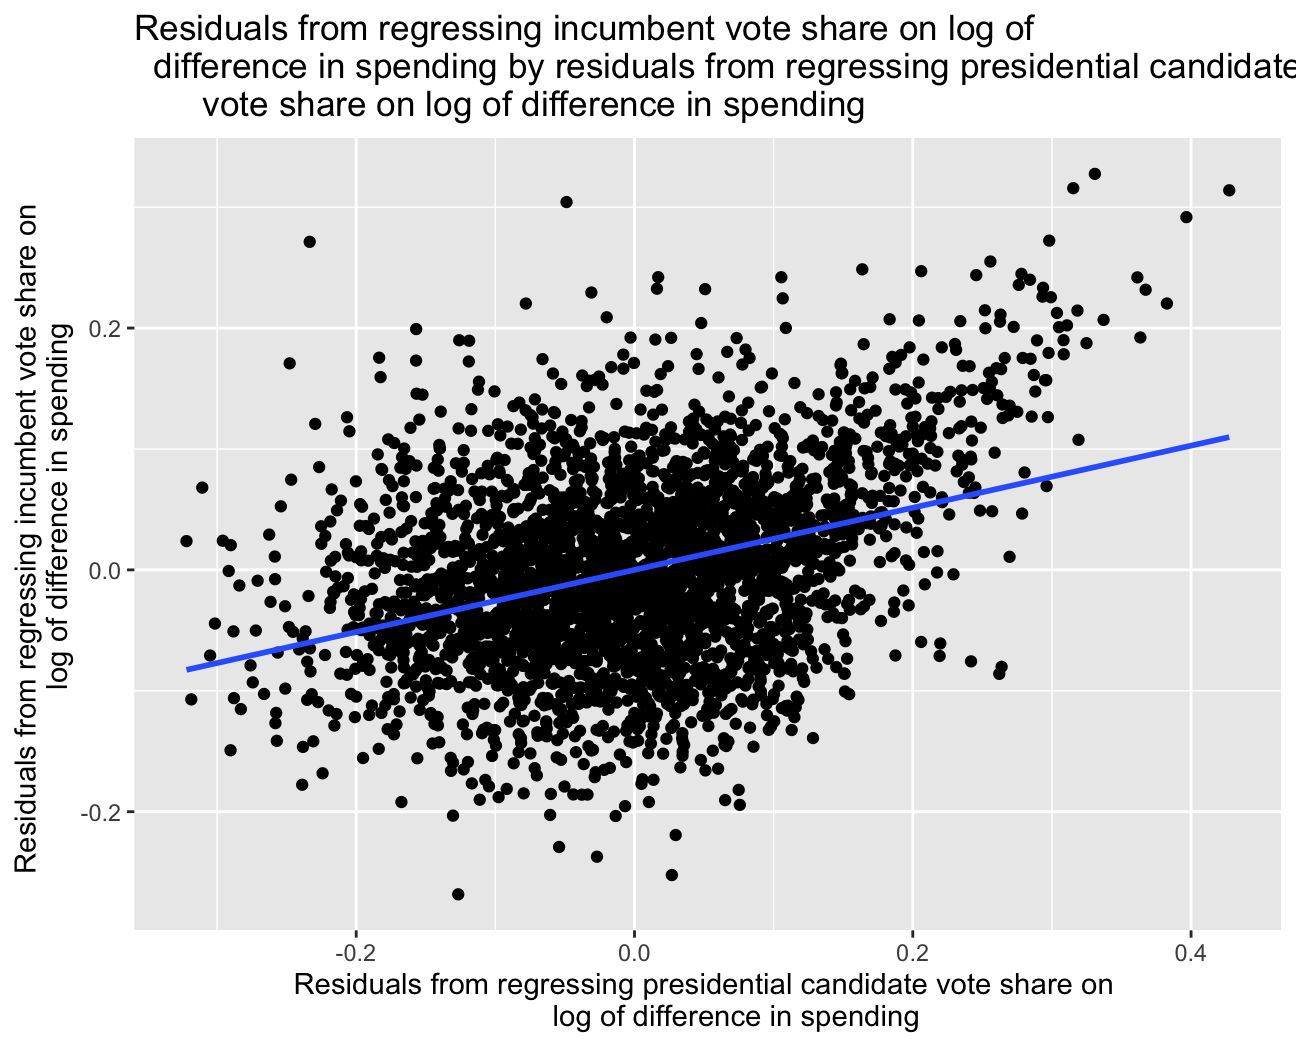
\includegraphics[scale=0.35]{problem4part2graph2}
		
		\item Write the prediction equation.
		
		I run the "summary" command again to get the regression coefficient values:
			\lstinputlisting[language=R, firstline=272, lastline=272]{PS03_answers_OS.R}
		
		The "summary" command produces the following output:
			\begin{verbatim}
			Residuals:
			Min       1Q   Median       3Q      Max 
			-0.25928 -0.04737 -0.00121  0.04618  0.33126 
			
			Coefficients:
			Estimate Std. Error t value Pr(>|t|)    
			(Intercept)                -1.942e-18  1.299e-03    0.00        1    
			residuals_presvote_difflog  2.569e-01  1.176e-02   21.84   <2e-16 ***
			---
			Signif. codes:  0 ‘***’ 0.001 ‘**’ 0.01 ‘*’ 0.05 ‘.’ 0.1 ‘ ’ 1
			
			Residual standard error: 0.07338 on 3191 degrees of freedom
			Multiple R-squared:   0.13,	Adjusted R-squared:  0.1298 
			F-statistic:   477 on 1 and 3191 DF,  p-value: < 2.2e-16
		\end{verbatim}
		
		From the output above:
		
		$\hat{\beta}_0$ (intercept) = -1.942e-18
		
		$\hat{\beta}_1$ (slope) = 2.569e-01
		
		\vspace{.5cm} Therefore:
		
		\textbf{		$\hat{residual from regressing voteshare on difflog}$ = (-1.942e-18) + (2.569e-01)(\textit{residual from regressing presvote on difflog}) + $\epsilon$}
		
	\end{enumerate}
	
	\newpage	

\section*{Question 5}
\noindent What if the incumbent's vote share is affected by both the president's popularity and the difference in spending between incumbent and challenger? 
	\begin{enumerate}
		\item Run a regression where the outcome variable is the incumbent's \texttt{voteshare} and the explanatory variables are \texttt{difflog} and \texttt{presvote}.	\vspace{.5cm}
		
		I regress \textit{voteshare} on \textit{difflog} and \textit{presvote} using the following commands:
		\lstinputlisting[language=R, firstline=286, lastline=288]{PS03_answers_OS.R}
		
		The "summary" command produces the following output:
		
			\begin{verbatim}
			Residuals:
			Min       1Q   Median       3Q      Max 
			-0.25928 -0.04737 -0.00121  0.04618  0.33126 
			
			Coefficients:
			Estimate Std. Error t value Pr(>|t|)    
			(Intercept)      0.4486442  0.0063297   70.88   <2e-16 ***
			inc.sub$difflog  0.0355431  0.0009455   37.59   <2e-16 ***
			inc.sub$presvote 0.2568770  0.0117637   21.84   <2e-16 ***
			---
			Signif. codes:  0 ‘***’ 0.001 ‘**’ 0.01 ‘*’ 0.05 ‘.’ 0.1 ‘ ’ 1
			
			Residual standard error: 0.07339 on 3190 degrees of freedom
			Multiple R-squared:  0.4496,	Adjusted R-squared:  0.4493 
			F-statistic:  1303 on 2 and 3190 DF,  p-value: < 2.2e-16
		\end{verbatim}
		
		\item Write the prediction equation.	\vspace{0.5cm}
		
		From the output above:
		
		$\hat{\beta}_0$ = 0.4486442
		
		$\hat{\beta}_1$ = 0.0355431
		
		$\hat{\beta}_2$ = 0.2568770
		
		Therefore:
		
\textbf{		$\hat{voteshare}$ = 0.4486442 + 0.0355431(\textit{difflog}) + 0.2568770(\textit{presvote}) + $\epsilon$}
		
		\item What is it in this output that is identical to the output in Question 4? Why do you think this is the case? \vspace{.5cm}
		
		From the output tables above, I see that the minimum, first quartile, median, third quartile, and maximum residuals are identical:
		
		\begin{verbatim}
			Residuals:
			Min       1Q   Median       3Q      Max 
			-0.25928 -0.04737 -0.00121  0.04618  0.33126 
		\end{verbatim}
		
		The residual standard errors are also identical:
		
		\begin{verbatim}
			Residual standard error: 0.07339 
		\end{verbatim}
		
		
		??????????????OK BUT WHY ARE THEY IDENTICAL??????????????????
		??????????????OK BUT WHY ARE THEY IDENTICAL??????????????????
		??????????????OK BUT WHY ARE THEY IDENTICAL??????????????????
		??????????????OK BUT WHY ARE THEY IDENTICAL??????????????????
		??????????????OK BUT WHY ARE THEY IDENTICAL??????????????????
		??????????????OK BUT WHY ARE THEY IDENTICAL??????????????????
		??????????????OK BUT WHY ARE THEY IDENTICAL??????????????????
		??????????????OK BUT WHY ARE THEY IDENTICAL??????????????????
		??????????????OK BUT WHY ARE THEY IDENTICAL??????????????????
		??????????????OK BUT WHY ARE THEY IDENTICAL??????????????????
		??????????????OK BUT WHY ARE THEY IDENTICAL??????????????????
		??????????????OK BUT WHY ARE THEY IDENTICAL??????????????????
		??????????????OK BUT WHY ARE THEY IDENTICAL??????????????????
		??????????????OK BUT WHY ARE THEY IDENTICAL??????????????????
		??????????????OK BUT WHY ARE THEY IDENTICAL??????????????????
		??????????????OK BUT WHY ARE THEY IDENTICAL??????????????????
		??????????????OK BUT WHY ARE THEY IDENTICAL??????????????????
		??????????????OK BUT WHY ARE THEY IDENTICAL??????????????????
		??????????????OK BUT WHY ARE THEY IDENTICAL??????????????????
		??????????????OK BUT WHY ARE THEY IDENTICAL??????????????????
		??????????????OK BUT WHY ARE THEY IDENTICAL??????????????????
		??????????????OK BUT WHY ARE THEY IDENTICAL??????????????????
		??????????????OK BUT WHY ARE THEY IDENTICAL??????????????????
		??????????????OK BUT WHY ARE THEY IDENTICAL??????????????????
		
	\end{enumerate}




\end{document}
